\chapter{Program Instructions}
\label{chap:program-instructions}

\section{Installation and Setup}

\fillin{Replace the commands below with the exact ones needed to run your program.}

\begin{enumerate}[itemsep=2pt]
  \item Install \fillin{Python version, for example Python 3.10 or later}.
  \item Clone or copy the project folder to your machine.
  \item Install the required libraries, for example:
  \begin{quote}
  \texttt{pip install \fillin{list of libraries, for example networkx matplotlib tkinter}}
  \end{quote}
  \item Place the dataset file, for example \fillin{dataset file name}, in the folder expected by the program, for example \fillin{data folder path}.
  \item Run the program with:
  \begin{quote}
  \texttt{python \fillin{main file name}}
  \end{quote}
\end{enumerate}

\section{Guidelines for Using the GUI}

\fillin{Adjust the steps below to match your actual GUI layout.}

\begin{enumerate}[itemsep=2pt]
  \item Open the program, the main window shows a map of the chosen area with all locations marked.
  \item Select a start location from the dropdown list, or click on it directly on the map.
  \item Select a goal location the same way.
  \item Choose which search algorithm to use from the algorithm menu.
  \item Press the search button to compute the route.
  \item The chosen route is drawn on the map, and the total cost, number of nodes explored, and processing time are shown in the results panel.
  \item To try the multi location feature, switch to the multi stop tab, add each location that must be visited, and press optimize to see the suggested visiting order.
\end{enumerate}

\section{Example Inputs and Outputs}

\fillin{Fill in a real example run of your program.}

\begin{table}[h!]
\centering
\caption{Example single route input and output}
\begin{tabular}{ll}
\toprule
Field & Value \\
\midrule
Start location & \fillin{location} \\
Goal location & \fillin{location} \\
Algorithm & \fillin{algorithm name} \\
Resulting path & \fillin{node sequence} \\
Total cost & \fillin{value} \\
Nodes explored & \fillin{value} \\
Processing time & \fillin{value} \\
\bottomrule
\end{tabular}
\end{table}

\begin{table}[h!]
\centering
\caption{Example multi location input and output}
\begin{tabular}{ll}
\toprule
Field & Value \\
\midrule
Start location & \fillin{location} \\
Locations to visit & \fillin{list of locations} \\
Original order & \fillin{sequence} \\
Optimized order & \fillin{sequence} \\
Total cost, original & \fillin{value} \\
Total cost, optimized & \fillin{value} \\
\bottomrule
\end{tabular}
\end{table}

\section{Screenshots of the System}

\fillin{Replace the placeholder images below with real screenshots of your running program.}

\begin{figure}[h!]
\centering
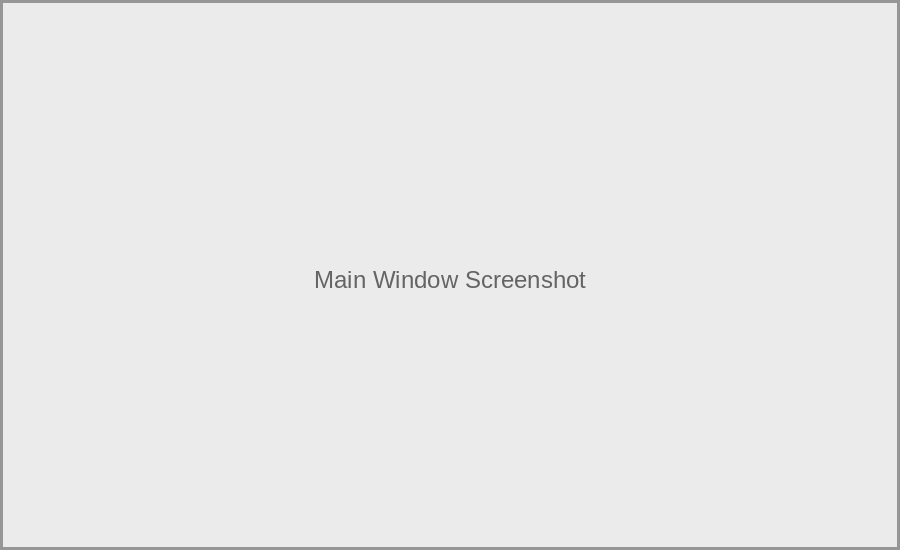
\includegraphics[width=0.85\textwidth]{images/screenshot_main_window.png}
\caption{Main window of the program showing the map and location list}
\label{fig:screenshot-main}
\end{figure}

\begin{figure}[h!]
\centering
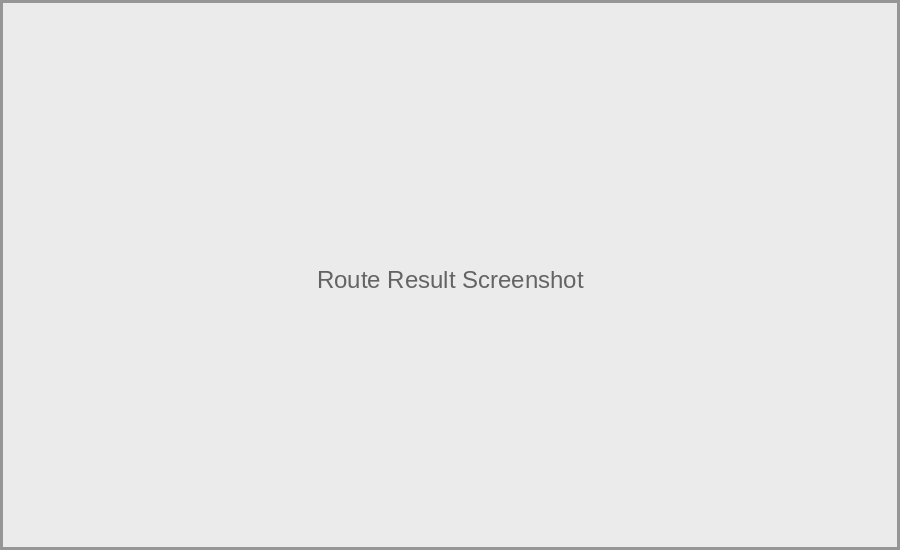
\includegraphics[width=0.85\textwidth]{images/screenshot_route_result.png}
\caption{Example of a computed route displayed on the map with cost and statistics}
\label{fig:screenshot-result}
\end{figure}

\begin{figure}[h!]
\centering
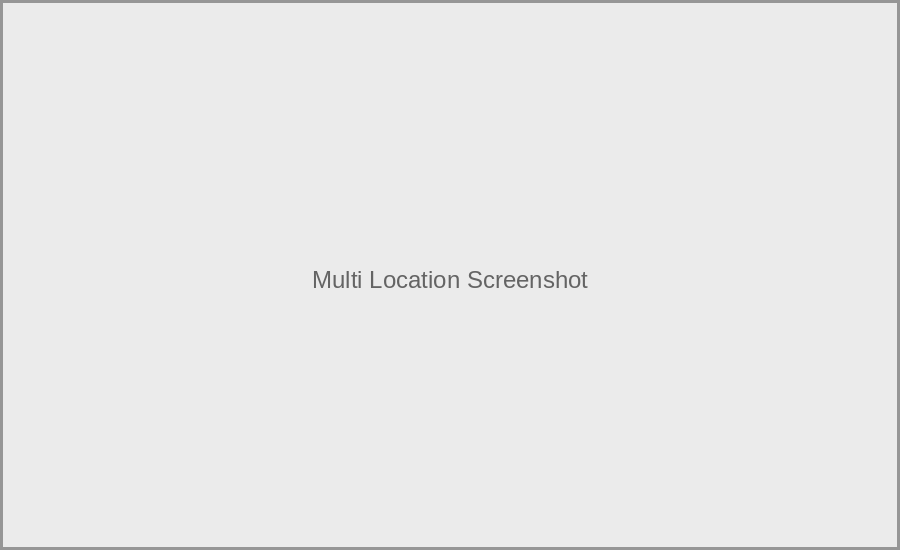
\includegraphics[width=0.85\textwidth]{images/screenshot_multi_location.png}
\caption{Multi location tab showing the original and optimized visiting order}
\label{fig:screenshot-multi}
\end{figure}
